\documentclass[12pt]{article}

\usepackage{ishn}

\makeindex[intoc]

\begin{document}

\hypersetup{pageanchor=false}
\begin{titlepage}
	\begin{center}
		\vspace*{1em}
		\Huge
		\textbf{III Topological Quantum Matter}

		\vspace{1em}
		\large
		Ishan Nath, Lent 2024

		\vspace{1.5em}

		\Large

		Based on Lectures by Prof. Benjamin B\'eri

		\vspace{1em}

		\large
		\today
	\end{center}
	
\end{titlepage}
\hypersetup{pageanchor=true}

\tableofcontents

\newpage

%lecture 1

\setcounter{section}{-1}

\section{Overview}%
\label{sub:o}

The \textbf{themes} in this course are:
\begin{itemize}
	\item Quantum matter, and topological order (TO).
	\item Quantum computing (QC), quantum error correction (QEC) and topological QC.
\end{itemize}

The \textbf{methods} are:
\begin{itemize}
	\item Mostly operator algebra (Pauli operators, fermion operators).
	\item Some field theory (second quantization and path integrals).
	\item A little band theory.
\end{itemize}

For notation, we have $N$ qubits, so $N$ sites. $X_j$, $Y_j$, $Z_j$ are the $X$, $Y$, $Z$ Pauli operators on the site $j$.

\newpage

\section{Quantum Ising Model}%
\label{sec:qim}

To recover a quantum Ising model, we can consider Hamiltonian
\[
H = - J \sum_{\langle i, j\rangle} Z_i Z_j - h \sum_j Z_j,
\]
for some $J > 0$. Then for an eigenstate $\ket{\{z_j\}}$,
\[
	H \ket{\{z_j\}} = E(\{z_j\}) \ket{\{z_j\}}.
\]
Also $\ket{\{z_j\}}$ are eigenstates of $Z_i$:
\[
	Z_i \ket{\{z_j\}} = z_i \ket{\{z_j\}}.
\]
This is quite boring; we just need to compute $E(\{z_j\})$. The \emph{transverse field Ising model}\index{transverse field Ising model} is given by replacing the last $Z_j$ with an $X_j$:
\[
H = - J \sum_{\langle i, j\rangle} Z_i Z_j - h \sum_j X_j.
\]
This Hamiltonian has a $\mathbb{Z}_2$ symmetry $P = \prod_j X_j$. This is because $X_j$ and $Z_j$ anticommute, giving $HP = PH$, and $P^2 = 1$. This corresponds to flipping all the spins, $P \ket{\{z_j\}} = \ket{\{-z_j\}}$.

If $J = 0$, then we have a ground state given by
\[
	\ket{\mathrm{GS}} = \bigotimes_{j = 1}^N \ket +_j = \ket{\mathbf{X}},
\]
where $X_j \ket{\mathbf{X}} = \ket{\mathbf{X}}$. Recall that
\[
\ket{\pm} = \frac{\ket{\uparrow} \pm \ket{\downarrow}}{\sqrt 2}.
\]
If $h = 0$, we have ground states
\[
	\ket{\Uparrow} = \bigotimes_{j = 1}^n \ket \uparrow_j, \qquad \ket\Downarrow = \bigotimes_{j = 1}^n \ket \downarrow_j,
\]
or any linear combination of these.

We want to analyse these ground states. For the first, note $P\ket{\mathbf{X}} = \ket{\mathbf{X}}$, and $\braket{\mathbf{X}|Z_j|\mathbf{X}}=0$, since $Z_j \ket + _j = \ket -_j$. This can be thought of as a \emph{paramagnet}\index{paramagnet}.

For the other ground state, $P \ket \Uparrow = \ket \Downarrow$, and $\braket{\Uparrow|Z_j|\Uparrow} \neq 0$. This can be thought of as a \emph{ferromagnet}\index{ferromagnet}.

Since $[H, P] = 0$, there exists a basis $\ket{\psi_{E, p}}$ with 
\[
	H \ket{\psi_{E,p}} = E_P \ket{\psi_{E,p}}, \qquad P\ket{\psi_{E,p}} = p \ket{\psi_{E,p}}.
\]
Consider the following ground state:
\[
	\ket{\mathrm{GS}_{\pm}} = \frac{\ket \Uparrow \pm \ket \Downarrow}{\sqrt 2}.
\]
Then this satisfies $P\ket{\mathrm{GS}_{\pm}} = \pm \ket{\mathrm{GS}_{\pm}}$, and $\braket{\mathrm{GS}_{\pm}|Z_j|\mathrm{GS}_{\pm}} = 0$.

To analyse this, we let $H = H_0 + \delta H$, where
\[
H_0 = - J \sum_{\langle i, j\rangle} Z_i Z_j, \qquad \delta H = - h \sum_j X_j.
\]
\subsection{Brillouin-Wigner Perturbation Theory}%
\label{sub:bwpt}

Let $H = H_0 + \delta H$, where $H_0 \ket n = E_n \ket n$ and $H \ket{\tilde n} = E_{\tilde n} \ket{\tilde n}$, the eigenstates.

For $h = 0$ there is a energy gap $\Delta > 0$ between the ground state and the first excited state. Let the ground state subspace be $S$, and $d = \dim S$, the levels or the ground state degeneracy.

We can write our particle number or projection operators as 
\[
P = \sum_{n \in S} \ket n \bra n.
\]
Then we can take $Q = \mathbbm{1} - P$.

Let $E_{\tilde m}$ be the perturbed GS energies, and $\ket{\tilde m^{(u)}}$ the unnormalised perturbed eigenstates. So $H \ket{\tilde m^{(u)}} = E_{\tilde m} \ket{\tilde m^{(u)}}$, and $P\ket{\tilde m^{(u)}} = \ket{\psi_{\tilde m}}$, which is normalized.

Now write out
\begin{align*}
(H_0 + \delta H) \ket{\tilde m^{(u)}} &= E_{\tilde m} \ket{\tilde m^{(u)}}, \\
(E_{\tilde m} - H_0)\ket{\tilde m^{(u)}} &= \delta H \ket{\tilde m^{(u)}} \implies (E_{\tilde m} - E_{\tilde n}) \braket{n|\tilde m^{(u)}} = \braket{n | \delta H | \tilde m^{(u)}}.
\end{align*}
This lets us write
\[
	\sum_{n \in S^{\perp}} \ket n \braket{n|\tilde m^{(u)}} = \sum_{n \in S^{\perp}} \frac{\ket n \bra n}{E_{\tilde m} - E_n} \delta H \ket {\tilde m^{(u)}}.
\]
So
\[
	Q \ket{\tilde m^{(u)}} = G \delta H \ket {\tilde m^{(u)}},
\]
which we can invert and write in terms of $\psi$ to get
\[
	\ket{\tilde m^{(u)}} = (\mathbbm{1} - G \delta H)^{-1} \ket{\psi_{\tilde m}}.
\]
For $\ket n \in S$,
\begin{align*}
	(E_{\tilde m} - E_0) \braket{n|\tilde m^{(u)}} &= \braket{n|\delta H(\mathbbm{1} - G \delta H)^{-1} | \psi_{\tilde m}} \\
						       &= \sum_{n' \in S} \braket{n|A^{(\tilde m)}|n'} \braket{n'|\tilde m^{(u)}}.
\end{align*}
We can think of the first term as $H_{nn'}^{\mathrm{eff}}$, and we can write $v_n^{(\tilde m)} = \braket{n|\tilde m^{(u)}}$.

% lecture 2

Once again, the perturbation is such that the ground state energy, once perturbed, is still away from the first excited energy $E_0 + \Delta$. This lets us write
\[
\sum_{n' \in S} H_{nn'}^{\mathrm{eff}}(E_{\tilde m}) v_{n'} = (E_{\tilde m} - E_0) v_n.
\]
When we write $H_{nn'}^{\mathrm{eff}}$, we introduce
\[
G^{(\tilde m)} = \sum_{n \in S^{\perp}} \frac{\ket n \bra n}{E_{\tilde m} - E_n}.
\]
Note that
\[
E_{\tilde m} - E_n = (E_0 - E_n) + (E_{\tilde m} - E_0),
\]
and the latter is small for small perturbations, so we can neglect this.

\subsection{Applications to Transverse Field Ising Model}%
\label{sub:atfim}

Recall that
\[
H = - J \sum_{\langle i, j\rangle} Z_i Z_j - h \sum_j X_j.
\]
Recall $P$, the product of $X_j$, is a symmetry, and we have ground states $S$ for the Hamiltonian $H_0$ spanned by
\[
	\ket{\mathrm{GS}_{\pm}} = \frac1{\sqrt 2} (\ket\Uparrow \pm \ket \Downarrow),
\]
where $P\ket{\mathrm{GS}_{\pm}} = \pm \ket{\mathrm{GS}_{\pm}}$. Then we can write
\begin{align*}
	\delta E_{\pm} &= \braket{\mathrm{GS}_{\pm} | \delta H(\mathbbm{1} - G \delta H)^{-1} | \mathrm{GS}_{\pm}} \\
		       &= \braket{\mathrm{GS}_{\pm} | \delta H| \mathrm{GS}_{\pm}} + \braket{\mathrm{GS}_{\pm} | \delta H G \delta H | \mathrm{GS}_{\pm}} \\
		       &\qquad + \braket{\mathrm{GS}_{\pm} |\delta H G \delta H G \delta H | \mathrm{GS}_{\pm}} + \cdots.
\end{align*}
First we look at $\delta H \ket{\mathrm{GS}_{\pm}}$. Note this is
\[
	-h \sum_j X_j \ket{\mathrm{GS}_{\pm}}.
\]
This has no overlap with $\ket{\mathrm{GS}_{\pm}}$, as the first has some spins flipped, and the latter has no spins flipped.

Consider now what $G$ does to $\delta H \ket{\mathrm{GS}_{\pm}}$. The latter is a sum of states, exactly one of which has a flipped spin. Hence when we compute it with $G$, it picks out the excited state and gives a term of
\[
\frac{1}{E_0 - E_n} = \frac{-1}{c J},
\]
for some constant $c$. Hence we get
\[
	G \delta H \ket{\mathrm{GS}_{\pm}} \sim \frac{h}{J} \sum_j X_j \ket{\mathrm{GS}_{\pm}}.
\]
The second $\delta H$ may undo the spin flip, giving
\[
	\braket{\mathrm{GS}_{\pm} | \delta H G \delta H | \mathrm{GS}_{\pm}} \sim - N \frac{h^2}{J} \braket{\mathrm{GS}_{\pm} | \mathrm{GS}_{\pm}}.
\]
This perturbation is independent of $p$. Moreover, the perturbation is of order $N$, which is scary. However it is fine after a bit of consideration; our ground states have energy at order $N$. To be more precise, we can start with $N$ finite and then send $N$ to infinity in our theory.

We can continue this, and look at the perturbations, and see they are independent of $p$ up to order $m < N$. However, eventually we get
\begin{align*}
	\braket{\mathrm{GS}_{\pm} | \delta H G \delta H \cdots G \delta H | \mathrm{GS}_{\pm}} &\to \frac{\delta E^{(m)}}{2} \braket{\mathrm{GS}_{\pm} \prod_{j = 1}^N X_j | \mathrm{GS}_{\pm}} \\
											       &= \pm \frac{\delta E^{(m)}}{2},
\end{align*}
where our perturbation depends on $p$. So the splitting energy is
\[
\delta E^{(\mathrm{split})} \sim \frac{h^{N}}{J^{n-1}} \sim J \left( \frac{h}{J} \right)^N,
\]
which is exponentially suppressed in $N$.

So the ground state degeneracy is exponentially accurate, but it is linearly unstable; it depends on the $\mathbb{Z}_2$ symmetry of the perturbation. Indeed, if $\delta H = h' Z_j$, and if our ground states are $\ket n \to \ket \Uparrow, \ket \Downarrow$, then
\[
\delta E_{\uparrow, \downarrow} = \pm h'.
\]
A few things to glean from the transverse field Ising model:
\begin{itemize}
	\item There is no more spontaneous symmetry breaking in the ground state. Let $\ket \psi$ be the exact ground state, for $N \gg 1$.

		Then $P \ket \psi = p \ket \psi$ is $\mathbb{Z}_2$ symmetric, hence since $P Z_i = - Z_i P$,
		\[
			\braket{\psi|Z_i|\psi} = 0.
		\]
	\item If $J \gg |h|$, we have a ferromagnet, with ground state degeneracy. If $J \ll |h|$, we have a paramagnet, with unique ground state.
	\item In the ferromagnetic case, if we let
		\[
			\ket{\psi_{\Uparrow,\Downarrow}} = \frac{\ket{\psi_+} \pm \ket{\psi_-}}{\sqrt 2},
		\]
		these are approximate ground states, with
		\[
			P\ket{\psi_{\Uparrow}} = \ket{\psi_{\Downarrow}} \implies \braket{\psi_{\Uparrow}|Z_j|\psi_{\Uparrow}} = M_0 \neq 0.
		\]
		What we can do is include a
		\[
		h' Z_j
		\]
		term in the perturbation, such that $\delta \eps_{\mathrm{split}} \ll h' \ll h$. Then,
		\[
			\lim_{h' \to 0} \lim_{N \to \infty} \braket{\psi | Z_j | \psi} = M_0.
		\]
		If we swap the limits, we get 0, since we remove the symmetry breaking interaction. This can be thought of as the first definition of spontaneous symmetry breaking.
	\item Another way to think of symmetry breaking is through correlation functions,
		\begin{align*}
			C_{|i-j|}^{(Z)} &= \braket{\psi|Z_i Z_j|\psi} - \braket{\psi|Z_i|\psi}\braket{\psi|Z_j|\psi} \to
			\begin{cases}
				M_0^2 & \text{ferromagnetic}, \\
				e^{-c|i = j|} & \text{paramagnetic}.
			\end{cases}
		\end{align*}
		Subtracting $\braket{\psi|Z_i|\psi}\braket{\psi|Z_j|\psi}$ just removes zero, but this is useful so that $C_{|i-j|}^{(O)} \to 0$ for large $|i-j|$, and $O = Z, X, Y$. This behaviour shows that $C_{|i-j|}^{(Z)}$ has long-range interactions in the ferromagnetic phase. In the paramagnetic there is no such order, giving a disordered phase.
\end{itemize}

\newpage

\section{Surface Codes}%
\label{sec:sc}

Our motivation is a sort of master formula for Pauli operators:
\[
\left( \prod_{j \in M} X_j \right) \left( \prod_{j \in M'} Z_j \right) = (-1)^{|M \cap M'|} \left( \prod_{j \in M'}Z_j \right) \left( \prod_{j \in M} X_j \right).
\]
This can be proven by pulling each $X_j$ through individually: it commutes with all $Z_{j'}$ except if $j = j'$, in which case it anticommutes.

To define surface codes, we consider a 2D square lattice, where qubits are placed on each edge of the lattice. We can represent operators by lines through these edges: if they are parallel to the edge, they correspond to $Z_i$, whereas if they are orthogonal they correspond to $X_i$.

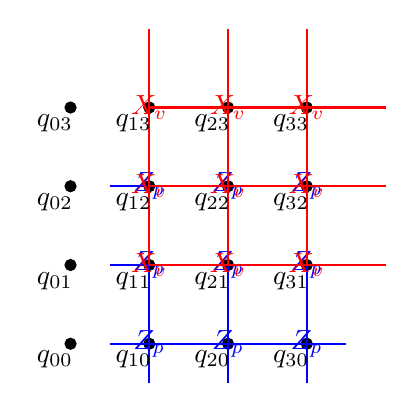
\begin{tikzpicture}
    % Draw lattice
    \foreach \x in {0,1,2,3} {
        \foreach \y in {0,1,2,3} {
            \filldraw (\x,\y) circle (2pt);
        }
    }
    
    \foreach \x in {0,1,2} {
        \foreach \y in {0,1,2} {
            % Plaquette (Z-type) operator
            \draw[blue, thick] (\x+0.5,\y) -- (\x+1.5,\y);
            \draw[blue, thick] (\x+1,\y-0.5) -- (\x+1,\y+0.5);
            \node[blue] at (\x+1,\y) {$Z_p$};
        }
    }
    
    \foreach \x in {1,2,3} {
        \foreach \y in {1,2,3} {
            % Vertex (X-type) operator
            \draw[red, thick] (\x,\y) -- (\x+1,\y);
            \draw[red, thick] (\x,\y) -- (\x,\y+1);
            \node[red] at (\x,\y) {$X_v$};
        }
    }
    
    % Label qubits
    \foreach \x in {0,1,2,3} {
        \foreach \y in {0,1,2,3} {
            \node at (\x-0.2,\y-0.2) {$q_{\x\y}$};
        }
    }
\end{tikzpicture}

The \emph{plaquette operators}\index{plaquette operators} are the four lines around a face, corresponding to
\[
\prod_{j \in p} Z_j = B_p.
\]
The \emph{vertex operators}\index{vertex operators} are the four lines around a vertex, corresponding to
\[
\prod_{j \in v} X_j = A_v.
\]

A \emph{surface code}\index{surface code} is simply a system where the Hamiltonian is
\[
H = - J_A \sum_v A_v - J_B \sum_p B_p.
\]
Note that $[A_v, B_p] = 0$, because they have intersection either $0$ or $2$, and by our master formula. Hence also
\[
	[A_v, H] = [B_p, H] = 0.
\]
Also $A_v^2 = \mathbbm{1} = B_p^2$, so the eigenvalues are in $\{\pm 1\}$.

Our task is now to find more integrals of motion, and eigenstates $\ket n$. For example we can consider
\[
\prod_{v \in V} A_v \prod_{p \in P}B_p,
\]
which is an integral of motion but is not independent of the $A_v, B_p$ we have already seen. One example is
\[
\chi_M = \prod_{j \in M} X_j.
\]
Can we pick $M$ such that $\chi_M$ is an integral of motion? To commute with all of the $B_p$, then the $M$ must represent a path without endpoints (insert picture).

One example of a loop is $A_v$. Moreover, we can multiply different $A_v$ to find larger loops: if we multiply the $A_v$ in a $3 \times 3$ region, we find a $3 \times 3$ loop.

We can now introduce \emph{path deformation}\index{path deformation}. Consider taking a path, and multiplying it by an $A_v$. This gives us another path, e.g.
\[
\prod_{j \in \tilde \gamma} X_j \cdot A_v = \prod_{j \in \tilde \gamma'} X_j.
\]
We can now talk about \emph{contractible loops}\index{contractible loops}: we can multiply it by a set of $A_v$ such that the path disappears.

We will now see where topology comes in.

% lecture 3

\begin{definition}
	A \emph{manifold}\index{manifold} is a space which is locally Euclidean, for example a sphere or a torus.

	The \emph{first Betti number}\index{first Betti number} of $\mathcal M$, $\mathcal{B}_1$ is the number of noncontractible independent paths of $\mathcal{M}$.
\end{definition}
Note that the Betti number is a topological invariant.

Consider our surface code on a manifold $\mathcal{M}$: and take $\tilde \gamma_1, \tilde \gamma_2, \ldots$ the non-contractible independent paths. Then
\[
\bar X_j = \chi_{\tilde \gamma_j}= \prod_{i \in \tilde \gamma_j} X_i \neq \prod_{v \in V} A_v,
\]
for some $v$, hence this is independent. Note that $\bar X_j^2 = \mathbbm{1}$, so it has eigenvalues in $\{\pm 1\}$.

Moreover, we can also consider
\[
\bar Z_j = \prod_{i \in \tilde \gamma_i} Z_i.
\]
Again $\bar Z_j^2 = \mathbbm{1}$, but more importantly
\[
\bar X_i \bar Z_j = (-1)^{\delta_{ij}} \bar Z_j \bar X_i,
\]
like Pauli operators. We will find that our eigenstates are denoted by
\[
	\ket n = \ket{\{a_v\}, \{b_p\}; \bar z_1, \bar z_2, \ldots, \bar z_{\mathcal{B}_1}},
\]
where we either take $\{\bar X_i\}$ or $\{\bar Z_i\}$. We have not shown yet that these are the complete quantum numbers. However what we do know is that the energy is independent of $\{\bar Z_j\}$, hence the ground state degeneracy is
\[
2^{\mathcal{B}_1}.
\]
\subsection{Surface Code Excitations}%
\label{sub:sce}

The ground states are where $a_v = b_p = 1$, since $J_A, J_B > 0$. The excitations come in the form when some $a_v = -1$, or some $b_p = -1$, and combinations.

Denote one of the ground states as $\ket \psi$, and consider $Z_\alpha \ket \psi$, where $\alpha$ has some boundary. Consider what $A_v$ evaluates on this state.

If $v$ is the vertex for which $\alpha$ ends on, then we find
\[
A_v (Z_\alpha \ket \psi) = - Z_\alpha (A_v \ket \psi) = - Z_\alpha \ket \psi,
\]
so this state now has $a_v = -1$.

We can think of these lines as \emph{particles}\index{particles}. In particular, if $a_v = -1$, we think of this as an `e' particle, with energy $2 J_A$. If we have $M$ e particles, the energy is $2M J_A$.

Moreover,
\[
\prod_{p \in P} B_p Z_\alpha \ket \psi = Z_\alpha \prod_{p \in P} B_p \ket \psi = Z_\alpha \ket \psi.
\]
So we only care about the endpoints of the strings, and not about the paths taken between the endpoints.

If $b_p = -1$, then we have `m' particles, with energy $2 J_B$.

\subsection{Particle Exchange}%
\label{sub:pe}

We will look at particle exchange as a dynamical process, and we look at the exchange only.

The first thing we will focus on is identical particles, with initial configuration the same as the final configuration. We strip away:
\begin{itemize}
	\item Interactions, so particles are ``far'' apart.
	\item Local details, such as potentials.
\end{itemize}
If particles are far apart, we are considering nonintersecting worldlines, and as we only care about local details we only think about topological invariant features.

We will sit in $2 + 1$ dimensions, and can view them in the following pictorial way, as braids (insert picture of braids somehow???).

These braids also form a group: we can compose exchanging particles. Moreover, we have inverses.

Let the set of \emph{braids}\index{braid} be $B_N$, where we have $N$ strands. Then,
\begin{itemize}
	\item $\sigma_i, \sigma_j \in B_N \implies \sigma_i \sigma_j \in B_N$.
	\item $1 \in B_N$, $\sigma_i^{-1} \in B_N$.
\end{itemize}

These $\sigma$ and their inverses form the \emph{braid group}\index{braid group}. This is not commutative. However what is true is that
\[
\sigma_j \sigma_{j+1} \sigma_j = \sigma_{j+1} \sigma_j \sigma_{j+1},
\]
\[
	\sigma_j \sigma_i = \sigma_i \sigma_j \text{ if } |i - j| = 2.
\]
We can also talk about distinguishable particles, where particles need to end up as the same particle they started with. If $\sigma_{a_i}$ is the swapping of two adjacent $a$'s in position $i$ and $i + 1$, this same action does not act appropriately on an $a$ and a $b$ in those positions.

In this case, we need to do $\sigma_{a_i}^2$, to end up with the same particles. This move is denoted as $\mu_{ab}$.

Moreover in 3D, the overpass and underpass are topologically equivalent, so $\sigma_i^2$. In this case, how the particles move do not matter, only where they end up. Hence the underlying group is $S_N$.

To each exchange $\sigma_j$, we assign a unitary operator $U(\sigma_j)$. This can be thought of as the topological part of the time-evolution, during particle exchange.

Moreover, we require it to be a representation, so
\[
U(\sigma_j) U(\sigma_i) = U(\sigma_j \sigma_i).
\]
This gives a unitary representation of the braid group $B_N$. We may have \emph{abelian representations}\index{abelian representation}
\[
U(\sigma_j) = e^{i \theta_j} \in \mathsf{U}(1),
\]
If we use the first relation for the braid group,
\[
e^{2i \theta_j} e^{i \theta_{j+1}} =  e^{2i \theta_{j+1}} e^{i \theta_j} \implies e^{i\theta_j} = e^{i \theta_{j+1}} = e^{i\theta}.
\]
In 3D, $(e^{i\theta})^2 = 1$, so $e^{i\theta} \in \{\pm 1\}$, giving the familiar bosons and fermions.

However in 2D, we have $\sigma_j^2 \neq \mathbbm{1}$, so $\theta$ can be any value. This gives us \emph{anyons}\index{anyons}, or in this case \emph{abelian anyons}.

Graphically, the clockwise exchange is $e^{i\theta}$ times doing nothing.

For distinguishable particles, $U(\mu_{ab}) = e^{i 2\theta_{ab}}$.

We can also have non-abelian reprsentations, so
\[
U(\sigma_i \sigma_j) = U(\sigma_i) U(\sigma_j) \neq U(\sigma_j) U(\sigma_i) = U(\sigma_j \sigma_i).
\]

% lecture 4

\subsection{Particles Statistics in Surface Codes}%
\label{sub:pssc}

Consider two anyons $e$ and $m$. If the anyon is at vertex $v$, then we can successively move it by applying $Z_j$ with $j \in v$. This moves $a_v = 1$ and the start of the anyon to an adjacent vertex.

Applying $Z_{\alpha_1}$ for successive applications of a path, the particles start point moves along the path.

We can consider a similar operation for $m$ particles. Consider our starting point, which is an $e$ and an $m$ particle, separated.

Now consider encircling the $m$ particle with the $e$ particle clockwise, by doing a loop. Let $\mathcal{Z}_{\alpha}$ be the $e$ particle, and $\mathcal{X}_{\beta}$ the $m$ particle. Moreover Let $\mathcal{Z}_{\mathrm{loop}}$ be the encircling loop. The initial state is
\[
\mathcal{Z}_{\alpha} \mathcal{X}_{\beta} \ket \psi.
\]
Consider $\mathcal{Z}_{\mathrm{loop}}$ times the same state. Note that
\[
\mathcal{Z}_{\mathrm{loop}} \mathcal{X}_\beta = - \mathcal{X}_\beta \mathcal{Z}_{\mathrm{loop}},
\]
as they intersect at one point, and
\[
\mathcal{Z}_{\mathrm{loop}} \ket \psi = \ket \psi
\]
since this is a loop. So
\[
\mathcal{Z}_{\mathrm{loop}} \mathcal{Z}_\alpha \mathcal{X}_\beta \ket \psi = - \mathcal{Z}_\alpha \mathcal{X}_\beta \ket \psi.
\]
So encircling the $e$ and the $m$ gives us a sign change to $-1$. These are bosons, or \emph{mutual semions}\index{mutual semions}, as encircling gives $\pi/2$ rotation.

\subsection{Charge-Flux Composites}%
\label{sub:cfc}

Recall we said that $\mathsf{U}(g)$ is the `topological part' of evolution, for some $g \in B_N$. We can write down
\begin{align*}
	\braket{\{\mathbf{x}_j(t_f)\} | T \exp( - i/h \int_{t_i}^{t_f} \diff t\, \hat H(t) | \{\mathbf{x}_j(t_i)\} } = \int_{\{\mathbf{x}_j(t_f)\} \leftarrow \{\mathbf{x}_j(t_i)\}} \mathcal{D}\{\mathbf{x}_j\} \, \exp(i/h S[\{\mathbf{x}_j\}]),
\end{align*}
where
\[
S = \int_{t_i}^{t_f} \diff t\, L.
\]
This is the \emph{path integral}\index{path integral}.

To prove this: If we denote the transition operator as $U(t_f, t_i)$, hen we introduce time slices $\Delta t$. Then,
\[
U(t + \Delta t, t) = U(p)U(x) + \mathcal{O}(\Delta t^2).
\]
Then we can insert the identity
\[
\mathbbm{1} = \int \diff x \diff p \, \ket x \bra x \ket p \bra p.
\]
For our case, we are considering elements of the braid group, so $\{\mathbf{x}_j(t_f)\} = \{\mathbf{x}_j(t_i)\}$. So we can classify $\{\mathbf{x}_j(t)\}$ with the braids $g \in B_N$ for which they are topologically equivalent.

Suppose our action decouples as
\[
	S[\mathbf{x}_j(t)] = S_0[\{\mathbf{x}_j(t)\}] + \hbar W(g),
\]
a local part plus a topological part. Then we can write the time evolution as
\[
	\sum_{g \in B_N} e^{i W(g)} \int_{\{\mathbf{x}_j(t)\} \in g} \mathcal{D} x \, \exp \left( \frac ih S[\{\mathbf{x}_k\}] \right).
\]
\subsection{Aharonov-Bohm and Aharonov-Casher}%
\label{sub:acab}

We work in two dimensions, with one type of particle of charge $q$ and an electromagnetic field. The Lagrangian is given by
\[
L = L_0 - q(\vphi - \mathbf{\dot x} \cdot \mathbf{A}).
\]
Consider a flux $\Phi$ piercing the plane at a fixed point $\mathbf{X}$, with $\vphi = 0$.

Then, for a loop $\mathbf{x}$ encircling $\mathbf{X}$ $n$ times, the action is
\[
	S[\mathbf{x}] = S_0 + q \int \diff t\, \mathbf{\dot x} \cdot \mathbf{A} = S_0 + q \oint \diff \mathbf{x} \cdot \mathbf{A} = S_0 + q n \Phi.
\]
This is the \emph{Aharonov-Bohm effect}\index{Aharonov-Bohm effect}.

Now suppose that the flux is situated at $\mathbf{X}(t)$. Then
\[
\mathbf{A}(\mathbf{x}) = \mathbf{A}_f(\mathbf{x}_k - \mathbf{X}(t)),
\]
where $\mathbf{A}_f$ is the potential for a flux at the origin, seems to give a good potential. However this is time-dependent, so
\[
\mathbf{E} = - \partial_t \mathbf{A} = (\mathbf{\dot X}_f \cdot \nabla)\mathbf{A} \neq 0.
\]
To remedy this, let $\phi = \mathbf{\dot X}_f \cdot \mathbf{A}$, which gives
\[
\mathbf{E} = - \partial_t \mathbf{A} - \nabla \phi = - \mathbf{\dot X}_f \times \mathbf{B},
\]
which vanishes at $\mathbf{x} \neq \mathbf{X}_f$. So,
\[
L = L_0 - q (\mathbf{\dot X}_f - \mathbf{\dot x}) \cdot \mathbf{A}_f(\mathbf{x} - \mathbf{X}_f).
\]
This also gives a phase $W[n] = q n \Phi/\hbar$ when circled $n$ times. This is the \emph{Aharonov-Casher effect}\index{Aharonov-Casher effect}.

\subsection{Charge-Flux Composites}%
\label{sub:cfc}

Suppose a particle $\mathbf{x}_j$ has a charge $q_j$ and flux $\Phi_j$ at some distance $\delta \mathbf{x}_j$ from the charge. The charge-flux interaction is
\[
L_I = -\sum_{j, k} q_j(\mathbf{\dot X}_k - \mathbf{\dot x}_j) \cdot \mathbf{A}_k(\mathbf{x}_j - \mathbf{X}_k).
\]
Suppose particle $j$ encircles particle $k$. Then from the two effects together, the change in encircling phase is
\[
e^{2 i \theta_{jk}} = e^{i/\hbar(q_j \Phi_k + q_k \Phi_j)}.
\]
If the particles are identical, the exchange phase is
\[
e^{i \theta} = e^{i/\hbar(q \Phi)}.
\]
Suppose we have a spin $J$ operator, and rotate about $z$. Then the operator is
\[
R(\alpha) = \exp( i/\eta \cdot \alpha J_z).
\]
Note $J_z/\hbar$ is a diagonal matrix which has half-integer elements if the spin if a half-integer, and integer otherwise. So, $R(2\pi) = \pm 1$ if these particles are bosons or fermions, and $R(2 \pi) = e^{i\theta}$.

In this model, doing a $2 \pi$ rotation gives
\[
R(2 \pi) = e^{i/\hbar \cdot (q \Phi)} = e^{i \theta},
\]
the exchange phase.

Suppose we have anyons $(q_1, \Phi_1)$ and $(q_2, \Phi_2)$, and then bring them close to each other. If we squint and only care about long-distance physics, then these become an anyon with state $(q_1 + q_2, \phi_1 + \phi_2)$.

In particular, bringing together $(q_1, \Phi_1)$ and $(-q_1, -\Phi_1)$ gives the \emph{identity particle}\index{identity particle}, or nothing. We can tikz this out (do this later!!!!)

If we denote by $\times$ as fusion, then in surface codes, $e \times e = 1$.

\subsection{Ground State Degeneracy and Topology}%
\label{sub:gsdt}

We now claim that the ground state knows about what anyons are possible.

Consider the torus, with two non-contractible loops $\gamma_1$ and $\gamma_2$. We consider a process, starting with $T_1, T_2$ that create an anyon/anti-anyon pair, drag the anyon along $\gamma_1, \gamma)2$, and then reannihilate them.

Doing this, we end up back in the ground state. We now examine the operator
\[
T_2^{-1} T_1^{-1} T_2 T_1.
\]
Consider the braid lines of the anyons/anti-anyons for this operator. It consists of only one pair of anyons encircling, so the end result is the encircling phase $e^{i 2 \theta}$, multiplied by doing nothing.

% lecture 5

Recall that $T_i$ take the ground state to the ground state: hence they must have a ground-state diagonal block in their decomposition. Let $\ket{\psi_\alpha}$ be such that
\[
	T_2 \ket{\psi_\alpha} = e^{i \alpha} \ket{\psi_\alpha}.
\]
Then from the fact about $T_2^{-1}T_1^{-1}T_2T_1 = e^{i2\theta}$, we find that
\[
	T_2 T_1 \ket{\psi_\alpha} = e^{2 i \theta} T_1 T_2 \ket{\psi_\alpha} = e^{2i\theta + i \alpha} T_1 \ket{\psi_\alpha},
\]
so $T_1 \ket{\psi_\alpha}$ is yet another eigenstate with eigenvalue $e^{2i\theta + i\alpha}$. If $e^{2i\theta} \neq 1$, these have different eigenvalues, so $\ket{\psi_\alpha}$ is perpendicular to $T_1 \ket{\psi_\alpha}$.

Moreover, we find $T_1^{j}\ket{\psi_\alpha}$ for $j = 0, \ldots, m-1$ are orthogonal if $e^{2i\theta j} \neq 1$ for $j \in \{1, 2, \ldots, m\}$. For a finite ground state degeneracy, we need $n$ and $m$ such that $2 \theta m = 2 \theta n$, so $\theta = \frac nm \pi$.

In this case, the ground state degeneracy is at least $m$. For a more complicated manifold with $g$ handles, the ground state degeneracy is at least $m^{g}$.

We can do a similar thing when there are more than one particles, e.g. $e$ and $m$ particles.

\newpage

\section{Chern-Simons Theory}%
\label{sec:cst}

In this theory,
\[
L = L_0 + \int \Diff2x \, \mathcal{L},
\]
where
\[
\mathcal{L} = \mathcal{L}_{\mathrm{CS}} - j^{\alpha} a_\alpha, \qquad \mathcal{L}_{\mathrm{CS}} = \frac{\kappa}{2} a^{\alpha} \eps^{\alpha\beta\gamma} \partial_\beta a_\gamma = \frac{\kappa}{2} a(\eps \partial a),
\]
and
\[
j^0 = \sum_{j = 1}^N q_j \delta(\mathbf{x} - \mathbf{x}(t)), \qquad \mathbf{j} = \sum_{j = 1}^{N} q_j \mathbf{\dot x}_j \delta(\mathbf{x} - \mathbf{x}_j(t)),
\]
which gives $\partial_\alpha j^\alpha = 0$. We check that it is a gauge theory. Say $a \to a + \partial \Lambda$. Then note $\eps \partial \partial = 0$, so
\[
\delta \mathcal{L} = \left( \frac{\kappa}{2} \partial \Lambda (\eps \partial a) - j \partial \Lambda\right) = \partial \left( \frac{\kappa}{2} \Lambda(\eps \partial a) - j \Lambda \right) + (\partial j)\Lambda = 0.
\]
\subsection{CS Flux Attachment}%
\label{sub:csf}

Consider $a \to a + \delta a$. We find that
\[
\delta a(\eps \partial a) + (a \eps \partial \delta a) = 2 \delta a( \eps \partial a) + \partial(\cdots).
\]
Hence
\[
	\partial S_{\mathcal{L}} = \int \Diff 3 x \delta a[\kappa(\eps \partial a)- j] = 0 \implies j = \kappa \eps \partial a.
\]
Hence $j^0 = \kappa \eps^{0\alpha\beta} \partial_\alpha a_\beta = \kappa b$. Here $b$ is the CS magnetic field. Consider a particle at a position $\mathbf{x}_\ell$, and a charge $q_\ell$. We integrate the charge over a space $\Omega_\ell$, to find
\[
q_\ell = \kappa \Phi_\ell \implies \Phi_\ell = \frac{q_\ell}{\kappa}.
\]
We claim that if we know $j^0 = \kappa b$ and $\partial_\alpha j^\alpha = 0$, then we get the equations of motion.

\subsection{Quantum Flux Attachment}%
\label{sub:qfa}

First we write
\begin{align*}
	\mathcal{L}_{\mathrm{CS}} &= \frac{\kappa}{2} \left[ a^0 \eps^{0\alpha\beta} \partial_\alpha a_\beta + a_\alpha \eps^{\alpha\beta0} \partial_\beta a_0 + a_\alpha \eps^{\alpha0\beta} \partial_0 a_\beta\right] \\
				  &= \kappa a_0 b + \mathcal{L}_{\mathrm{CS}}(a_0 \to 0) + \partial(\cdots).
\end{align*}
So quantum mechanically, we want to minimize a term involving
\[
	\int \mathcal{D} a_0 \, e^{\frac{i}{\eta} S[a_0]},
\]
where
\[
	S[a_0]= \int \Diff 3 x \, a_0(\kappa \eps^{0 \alpha\beta} \partial_\alpha a_\beta - j^0) = \int \Diff3x\, a_0(\kappa b- j^0).
\]
So using the fact that $\int \diff a \, e^{iax} \propto \delta(x)$, we find $\delta(\kappa b - j^0)$. Hence $j^0 = \kappa b$ is enforced, and as charge is conserved we find $j = \kappa\eps \partial a$.

Encircling two particles $k$ and $\ell$,
\[
	e^{i2 \theta_{k\ell}} = e^{\frac{i}{\hbar} (q_k \Phi_\ell + q_\ell \Phi_k)} = e^{\frac{i}{\hbar} 2 \frac{q_k q_\ell}{\kappa}} \implies \theta_{k\ell} = \frac{q_k q_\ell}{\kappa}.
\]
So we may think that we have found the encircling phase. But if we substitute back into our Lagrangian,
\[
\mathcal{L} = a \frac{\kappa}{2} (\eps \partial a) - j \alpha = - \frac{j \alpha}{2},
\]
so the Lagrangian is half that which we found in our flux-charge model, hence in actuality
\[
\theta_{k\ell} = \frac{q_k q_\ell}{2 \hbar \kappa}.
\]

\subsection{Charge Quantisation}%
\label{sub:cq}

Instead of looking at a path integral, we consider a wavefunction $\psi$ which, under a gauge transformation moves to $e^{\frac{i}{\hbar} q_0 \Lambda}\psi$, for $q_0$ the particle charge.

We assume that any other charge (in terms of the wavefunction) is $\tilde q = n q_0$, for some $n \in \mathbb{Z}$.

Consider a system on a torus, and a particle that loops once around the torus. The action is
\[
S_{\mathrm{curr}} = q \int \diff t \, \mathbf{\dot x} \cdot \mathbf{a} = q \oint \diff \bm{\gamma} \cdot \mathbf{a}.
\]
Under a gauge transformation $\mathbf{a} \to \mathbf{a} + \nabla \Lambda$, then
\[
\delta S_{\mathrm{curr}} = q \oint \diff \bm{\gamma} \cdot \nabla \Lambda = q (\Lambda(L) - \Lambda(0)).
\]
We do not need $\Lambda$ to be single valued, just $\psi$. Hence we can have $\Lambda(L) - \Lambda(0) = 2 \pi \hbar/q_0$, and find
\[
\delta S_{\mathrm{curr}} = 2 \pi \hbar \frac{q}{q_0}.
\]
This is worrying, as we expect our action to be gauge invariance. But we only need $e^{\frac{i}{\hbar} S_{\mathrm{curr}}}$ to be gauge invariant, showing that
\[
2 \pi \hbar \frac{q}{q_0} = 2 \pi \hbar n \implies q = n q_0.
\]
We now consider Chern-Simons theory on a closed manifold. Start with $\kappa b = j^0$, and say the theory lives on some 2-sphere $\Omega$. Integrating this over $\Omega$,
\[
\int_{\Omega} \kappa b = \int_{\Omega} j^0 = m q_0,
\]
since charge is quantized. Moreover, the LHS is also quantized in terms,
\[
\int_{\Omega} b = n \Phi_0, \qquad \Phi_0 = \frac{2 \pi \hbar}{q_0}.
\]
So we find that
\[
\kappa n \Phi_0 = m q_0.
\]
For the minimum number of non-zero particles, we find
\[
\kappa = \frac{q_0^2}{2 \pi \hbar} m,
\]
the minimum \emph{Chern-Simons level}\index{Chern-Simons level}. Hence
\[
q\theta = \frac{q_0^2}{2 \pi \hbar} = \frac{\pi}{m}.
\]
Earlier, we found that if $\theta = \frac{n}{m}\pi$, then the ground state degeneracy was at least $m^{g}$.

We can generalize to more particles. Say there are $M$ particle types. We introduce $M$ gauge fields $a_{I\alpha}$ for $I \in \{1, \ldots, M\}$, and also $M$ charges $q_I$. Then the Chern-Simons Lagrangian is
\[
\mathcal{L} = \mathcal{L}_{\mathrm{CS}} - \sum_{I = 1}^{M} j_I^{\alpha} a_{I\alpha},
\]
where
\[
\mathcal{L}_{\mathrm{CS}} = \frac{1}{4 \pi \hbar} \sum_{I, J} K_{IJ} a_I (\eps \partial a_J),
\]
where $K_{IJ} = K_{JI}$ is an integer and forms an invertible matrix.

We can show that
\[
\theta_{q, q'} = \pi q' K^{-1} q.
\]
For the surface code, we can show
\[
K =
\begin{pmatrix}
	0 & 2 \\ 2 & 0
\end{pmatrix},
\]
and the ground state degeneracy is at least $|\!\det K|^{g}$.

% lecture 6

\newpage

\section{Robustness of Topological Order}%
\label{sec:rot}

\subsection{Perturbed Surface Code}%
\label{sub:psc}

Consider a Hamiltonian
\[
H = H_0 + \delta H,
\]
where $H_0$ is our familiar surface code,
\[
H_0 =- J_A \sum_{v} A_v - J_B \sum_p B_p,
\]
and
\[
\delta H = \sum_j h O_j,
\]
where $O_j$ has local support, and the diameter of the support is at most $\xi < \infty$, where $\xi$ is a contant and $j \in \mathrm{supp} O_j$.

Here we are saying that the lengths in the surface code are $1$.

Moreover $O_j$ is bounded, i.e. the matrix element are of order $\mathcal{O}(1)$.

For $H$ and $H_0$ that satisfy these conditions, we call the pair a \emph{local Hamiltonian}\index{local Hamiltonian}.

To study perturbations, we recall the effective Hamiltonian
\[
	H^{(\mathrm{eff})} = \braket{n|\delta H(1 - G \delta H)^{-1} | n'}, \qquad G =\sum_{n \in S^{\perp}} \frac{\ket n \bra n}{E_{\tilde n} - E_n}.
\]
For $h = 0$, the ground state degeneracy is $4^{g}$, and the eigenbasis is
\[
	\ket n = \ket{\{a_v, b_p\}, \{\bar z_j\}}.
\]
Here $\bar Z_j$ are the operators around independent noncontractible loops.

We set $O_j = Z_j$ for concreteness, so $[O_j, Z_i] = 0$, and hence $[\bar Z_i, H] = 0$. In this case, $H^{(\mathrm{eff})}$ is some diagonal matrix.

Consider expanding the expression for the effective Hamiltonian. We get
\begin{align*}
	\braket{n | \delta H G \delta H G \cdots G \delta H | n'} \to \braket{n | \prod_{i \in I} \bar Z_i \prod_{p \in P} B_p | n},
\end{align*}
since each application creates a pair of $e$-particles, which must be cancelled out. If $I = \emptyset$, then we get something proportional to
\[
	J \left( \frac hJ\right)^{m} \braket{n| \prod_{p \in P}B_p |n'} = J \left( \frac hJ \right)^{m} \delta_{\{\bar z_j\} \{\bar z_j'\}}.
\]
This is independent of $\bar z_i$.

If $I \neq \emptyset$, we get
\[
	J \left( \frac hJ \right)^{m} \prod_{i \in I} \bar z_i \delta_{\{\bar z_j\} \{z_j'\}}.
\]
For the last perturbation to occur, we need $m \geq L$, then length of the smallest loop. Hence
\[
\delta E_{\mathrm{split}} \leq J \left( hJ \right)^{L}.
\]
This result generalizes to any $\delta H$ local.

Comparing to the transverse field Ising model,
\[
\delta E_{\mathrm{split}} \leq J \left( \frac hJ\right)^{N}.
\]
This is order $L^2$. If $[\delta H, P] = 0$, then we get symmetry preserving behaviour.

If $[\delta H, P] \neq 0$, e.g. $\delta H = h Z_1$, then we may have $\delta E_{\mathrm{split}} \sim h$.

\subsection{Topological Order}%
\label{sub:to}

A two-dimensional Hamiltonian is \emph{topologically ordered}\index{topological order} if:
\begin{itemize}
	\item $H$ is gapped.
	\item It has topological ground state degeneracy.
	\item For any locally supported $A$, and ground states $\ket{\psi_j}$,
		\[
			\braket{\psi_j|A|\psi_i} = c_A \delta_{ij}.
		\]
\end{itemize}
These last two properties are required to hold up to $e^{-c L}$ for some $c > 0$.

We can verify that these hold for the unperturbed surface code. For the perturbed surface code we have verified 1 and 2, but not yet 3.

\subsection{Phases of Matter}%
\label{sub:pm}

Consider a Hamiltonian $H(g)$, where $g$ are some parameters. Say $H(0) = H_0$, $H(1) = H_1$.

If we write out $H(g + \delta g) = H(g) + (H(g + \delta g) - H(g))$, and assume that $H(g)$ is local and gapped,

Topological ordering is a phase.

\begin{definition}
	Suppose $H_0, H_1$ are gapped and local. They are in the same \emph{topological phase}\index{topological phase} if there is a parametrization $g : [0, 1] \to H(g)$ that is continuous, such that $H(g)$ is gapped and local for all $g$, and $H(0) =H_0$, $H(1) = H_1$.
\end{definition}

This is a purely topological definition.

We say that $\ket{\psi_0} \sim \ket{\psi_1}$ if and only if $\ket{\psi_j}$ is a ground state of a gapped local $H_j$ such that $H_0 \sim H_1$. Alternatively, $\ket{\psi_1} = U \ket{\psi_0}$, for $U$ local unitary.

$U$ is \emph{local unitary}\index{local unitary} if it can be written as
\[
U_i = \prod_{j} W_j^{(i)},
\]
where the diameter of the support of $W_j^{(i)} < \ell < \infty$, and the supports are non-overlapping. Then $|U - U_1U_2| \leq e^{-a \ell}$.

These two definitions are equivalent if we consider \emph{quasilocal}\index{quasilocal} $H$, where
\[
H = \sum_j c_j O_j,
\]
where $O_j$ is bounded and $c_j \sim \exp (- \alpha_j \, \mathrm{diam} \, \mathrm{supp} \, O_j)$, where $a_j > 0$ is constant.

We can show that if $O_j$ is instead local, then $U^{\dagger} O_j U$ is quasilocal, as is $U O_j U^{\dagger}$:
% lecture 7
\[
U O_j U^{\dagger} = \sum_{i} c_{ji} \tilde O_{i},
\]
where $\tilde O_i$ is bounded and $c_{ji} \sim \exp (- \alpha_{ji} \, \mathrm{diam} \, (j \cup \, \mathrm{supp} \, \tilde O_i))$. This is some sort of smearing.

Now we can show the equivalence: Let $\ket{\psi_0}$ be the ground state of some $H_0 = \sum_j O_j$, and $\ket{\psi_1} = U \ket{\psi_0}$ for $U$ local unitary.

Consider a local unitary path $g \in [0, 1] \mapsto U(g)$ continuous, with $U(0) = \mathbbm{1}$, and $U(1) = U$. This is possible as the unitary group is a Lie group. Consider then
\[
	U(g) \ket {\psi_0}.
\]
This will then be the ground state of the Hamiltonian
\[
H(g) = U(g) H_0 U^{\dagger}(g) = \sum_j U(g) O_j U^{\dagger}(g).
\]
But we know the latter sums are quasilocal, so $H(g)$ is a quasilocal Hamiltonian, and moreover gapped as it is a unitary transformation of gapped $H_0$.

If we let $H_0 = H(0), H_1 = H(1)$, then $\ket{\psi_1}$ is the ground state of $H_1$ since
\[
	H_1 \ket{\psi_1} = U H_0 U^{\dagger} U \ket{\psi_0} = U H_0 \ket{\psi_0} = E U \ket {\psi_0} = E \ket{\psi_1}.
\]
Moreover $H_0 \sim H_1$, since we have constructed a given path. Hence $\ket{\psi_0} \sim \ket{\psi_1}$ in our first definition.

The other way is much harder. For this we need another definition of local unitary: $U$ is local unitary if and only if
\[
U = T \exp \left( \frac{i}{\hbar} \int_0^{T} \diff T \tilde H(t) \right),
\]
where the initial $T$ is time ordering, $\tilde H(t)$ is quasi local and $T$ is a finite constant. This can be shown to be equivalent to the other definition (as shown by Osborne).

Chen Lou and Wen showed that if $\ket{\psi_0} \sim \ket{\psi_1}$, then there exists $U$ local unitary with $\tilde H(t)$ build from $H(g)$ such that
\[
	\ket{\psi_1} = U \ket{\psi_0}.
\]
In general, if we have a set of ground states $\{\ket{\psi_0^{(i)}}\}$, $\{\ket{\psi_1^{(i)}}\}$, then there exists a local unitary $U$ such that
\[
	\ket{\psi_1^{(i)}} = \ket{\psi_0^{(i)}},
\]
where $U$ is independent of $i$ and the basis.

Indeed suppose that $U^{(i)}$ depends on $i$. Then by the definition of topological order,
\[
	O_A \delta_{i i'} = \braket{\psi_1^{(i')}|A|\psi_1^{i}} = \braket{\psi_0^{(i')}|U^{(i')\dagger}A U^{(i)} | \psi_0^{(i)}} \neq \delta_{i i'}.
\]
We can also consider $H_0 \sim H_0$ and $\ket{\psi_0^{(i)}} = U \ket{\psi_0^{(2)}}$. This is not always possible; indeed in our statement we only have the existence of an $U$ taking the set of ground states of $H_0$ to the set of ground states in $H_1$. But sometimes it can exist.

\subsection{Robustness of Braiding Statistics}%
\label{sub:rbs}

Let $H = H_0 + \delta H$, where
\[
H_0 = - J \left( \sum_v A_v + \sum_p B_p \right),
\]
and $\delta H$ local, i.e.
\[
\delta H = h \sum_j O_j.
\]
Then if $\ket \psi$ is a ground state of $H_0$, and $\ket{\tilde \psi}$ is a ground state of $H$, we have
\[
	\ket{\tilde \psi} = U \ket \psi.
\]
The parent Hamiltonian for $\ket{\tilde \psi}$ is either $H$, or $\tilde H = U H_0 U^{\dagger}$. However $H \neq \tilde H$.

For sake of illustration, take our base state $2e$ particles with energy $4J$, and $O_j = Z_j$. We have roughly $N^2$ of these unperturbed eigenstates, $\ket{n_{2e}}$. Thinking about matrix elements,
\begin{align*}
	\braket{n_{2e}'|\delta H|n_{2e}} \neq 0 \implies \text{the electrons are hopping}.
\end{align*}
This has order $h$, so our eigenstates spread out into a band of order $h$.

For $\tilde H$, we can write it as
\[
\tilde H = - J \left( \sum_v \tilde A_v + \sum_p \tilde B_p \right),
\]
where
\[
\tilde A_v = U A_v U^{\dagger}, \qquad \tilde B_p = U B_p U^{\dagger},
\] 
for $U$ local unitary. These are quasilocal. Now
\[
\tilde A_v \tilde B_p = U A_v U^{\dagger} U B_p U^{\dagger} = U(A_v B_p) U^{\dagger} = \tilde B_p \tilde A_v,
\]
so these commute, and are integrals of motion. Let their values be $\tilde a_v$, and $\tilde b_p$ in $\{-1, 1\}$. The same can be seen for the other integrals $\tilde Z$. Hence we find eigenstates
\[
	\ket{\tilde \psi_{\{\tilde a_v, \tilde b_p\}, \tilde z_j} } = U \ket{\{a_v, b_p\}, \{z_j\}}.
\]
Then $\tilde A_v$, $\tilde B_p$ have these as eigenstates, with eigenvalues $\tilde a_v, \tilde b_p$. However these are now quasilocal, instead of the completely local $A_v, B_p$.

Suppose that in $H_0$, two electrons were created by
\[
\mathcal{Z}_\alpha = \prod_{j \in \alpha} Z_j,
\]
some path. Then in $\tilde H$,
\[
\tilde{\mathcal{Z}}_\alpha = U \mathcal{Z}_\alpha U^{\dagger}.
\]
In the unperturbed phase, we saw that the $e$ and $m$ particles were mutual semions. In $\tilde H$, we still find that $e$ and $m$ are mutual semions, as the entire systems goes about a unitary transformation. In our interpretation, we need the smeared $e$ and $m$ particles to not intersect, hence they must be far apart.

% lecture 8

\newpage

\section{Surface Code with Boundaries}%
\label{sec:scwb}

A motivation is thinking about realisations of quantum devices. A torus may be physically realizable, but more often we will have a 2D grid with boundaries.

For most of the lecture the surface code will be the usual, where $Z_j$ is along the edges and $X_j$ is transverse; $A_v$ is around a vertex and $B_p$ is around a plaquette. The Hamiltonian is
\[
H = - J_A \sum_v A_v - J_B \sum_p B_p,
\]
with $J_{A, B} > 0$. The ground states we have seen are those with
\[
A_v \ket \psi = B_p \ket \psi = \ket \psi,
\]
i.e. $a_v = b_p = 1$. We also have path operators
\[
\mathcal{Z}_\alpha = \prod_{j \in \alpha} Z_j, \qquad \mathcal{X}_{\tilde \beta} = \prod_{j \in \tilde \beta} X_j.
\]
Then,
\[
\mathcal{Z}_\alpha A_v = (-1)^{|\alpha \cap v|} A_v \mathcal{Z}_\alpha,
\]
and similarly for $\mathcal{X}$ and $B$. How can we get integrals of motion in systems with boundaries?

The boundary may cut the vertices. For such vertices, again we let
\[
A_v = \prod_{j \in v} X_v = X_1 X_2 X_3,
\]
since there are only 3 paths surrounding the vertex. This gives away a key feature in this model: there are lots of paths given by $\mathcal{X}_{\tilde \alpha}$. However these paths still commute with plaquette operators, so
\[
\mathcal{X}_{\tilde \alpha} B_p = B_p \mathcal{X}_{\tilde \alpha}
\]
for all $p$. Does this give a new integral of motion? No; it can be written as the product of vertex operators. Moreover if we have a plaquette path $\mathcal{Z}_{\alpha}$, these do not commute with all $A_v$: for the vertices $v$ the path start and ends at, $A_v$ anticommutes with $Z_{\alpha}$.

There is also an analogous model where the boundary cuts the plaquette operators.

The first kind of boundary is a \emph{smooth boundary}\index{smooth boundary}, and the second is a \emph{rough boundary}\index{rough boundary}. These are defined up to some convention. Smooth can be thought of as a \emph{$X$ boundary}\index{$X$ boundary}, and rough as a \emph{$Z$ boundary}\index{$Z$ boundary}.

Suppose we have two $m$ particles in a smooth boundary. Their energy is $4 J_B$. As we move the particles, the energy stays constant, until one of the particles hits the boundary, at which point the particle vanishes and the energy is $2 J_B$. We say the boundary \emph{condenses}\index{condense} $m$ particles. Analogously, the rough boundary is an $e$ condensing boundary.

If we have a connected boundary, then all loops happen to be contractible as above. But when this is not the case, we may find non-contractible paths.

Non-contractible meaning under deformation: either multiplying by plaquette or vertex operators. This lets us move the path, or change its endpoint.

We consider some examples in $[-2, 2]^2 \setminus [-1, 1]^2$, a square with a hole. A path from the $\partial [-2, 2]^2$ to itself is not contractible, just by shifting the endpoint.

What about a path around the hole, $\tilde \alpha$ consisting of vertex paths? It is also contractible. One way to see this is by introducing a loop that joins our path to $\partial [-2, 2]^2$, then moving the endpoints.

What about $\tilde \gamma$, going from $\partial [-2, 2]^2$ to $\partial [-1, 1]^2$? This is non-contractible. To remove it from the system, we must move the two endpoints to meet. Detaching an endpoint corresponds to creating a particle, as it anticommutes with some operator.

What if the path $\tilde \gamma'$ around the hole was of plaquette operators? Then this is non-contractible, as the plaquette operators cannot cut the path like with $\tilde \alpha'$.

Denote
\[
\bar X_{1} = \mathcal{X}_{\tilde \gamma}, \qquad \bar Z_1 = \mathcal{Z}_{\tilde \gamma'}.
\]
These are integrals of motion which anticommute. We can label eigenstates with $\ket{\{a_v, b_p\}, \bar z_1}$. This gives a ground state degeneracy of 2.

This enumerates all possibilities up to deformation: anything is either a path or a loop.

What if the inner boundary was rough? Again $\tilde \alpha$ and $\tilde \alpha'$ are contractible. Moreover $\tilde \gamma'$ is also contractible, by moving it to the inner boundary, and we cannot connect the two boundaries. So here we have a ground state degeneracy of just 1.

What if we have $[-2, 2]^2$, where the top and bottom boundaries are smooth, and the left and right boundaries are rough? Despite looking simply connected, there are some degeneracies, for example the path $\tilde \gamma$ from top to bottom or path $\tilde \gamma'$ from left to right. These anticommute, giving ground state degeneracy of 2.

We can generalize for more general manifolds. Let $\beta_1$ be the number of independent non-contractible paths $\alpha_j$ with
\[
\bar Z_j = \prod_{i \in \alpha_j} Z_i,
\]
and with quantum number $\bar z_j \in \{-1, 1\}$. Then there exists $\bar X_j$ with
\[
\bar X_j \bar Z_i = (-1)^{\delta_{ij}} \bar Z_i \bar X_j.
\]
These are the dual lattice paths $\tilde \gamma_i$.

We can also ask about robustness of GSD, from $H = H_0 + \delta H$, where $\delta H$ is again local. The order of splitting is
\[
E_{\mathrm{split}} \sim J \left( \frac{h}{J} \right)^{L},
\]
where $L$ is the length of the shortest non-contractible path.

One tricky termination is the following. Consider again a square with top and bottom smooth, left and right rough.

% lecture 9

\newpage

\section{Quantum Error Correction}%
\label{sec:qec}

\subsection{Classical Error Correction}%
\label{sub:cec}

Our task is to store one bit $r \in \{0, 1\}$. For convenience we introduce $z = (-1)^{r}$, which can be thought of either $\{\uparrow, \downarrow\}$.

A logical operator is a \emph{bit flip}\index{bit flip}: $z \mapsto -z$. This can be caused by environmental effects.

Error correction can be done via redundancy, for example the \emph{classical repetition code}\index{classical repetition code}. In this case,
\[
z \to (z_1, \ldots, z_n) =
\begin{cases}
	\uparrow \cdots \uparrow & \uparrow \\
	\downarrow \cdots \downarrow & \downarrow
\end{cases}
\]
For this we take $n$ odd. The encoded logical operator is $z_i \mapsto - z_i$ for all $i$.

The first step is error detection: we measure all $z_j$. If they are not all equal, then an error has occurred.

For the error correction step, we flip the minority of spins. When does this procedure work? Let the number of errors be $q$. Then if $q < n/2$, error correction works. Otherwise, it gives a logical error.

The problem is that we do not know $q$. But we may know an error process, that is suspected. From this we can build an error model, for example a \emph{bit flip channel}\index{bit flip channel}
\[
z_j \mapsto
\begin{cases}
	-z_j & \text{probability } p, \\
	z_j & \text{probability } 1- p,
\end{cases}
\]
independently for all $j$. Hence $q \sim \Bin(n, p)$. Here $p$ is known as the \emph{error rate}\index{error rate}. The \emph{logical error probability}\index{logical error probability} is $\mathrm{Pr}_e = \mathrm{Pr}(q > n/2)$.

We know that $\mu_q = np$, $\sigma_q = \sqrt{n p (1 - p)}$, and hence from CLT, we can estimate
\[
	\frac{n/2 - \mu_q}{\sigma_q} = \frac{n(1/2 - p)}{\sqrt{n p(1-p)}} > \sqrt n (1 - 2p) > 0,
\]
for $p < 1/2$. This is positive, and grows with $n$. So we can find
\[
\mathrm{Pr}_e = \mathrm{Pr} (q > n/2) \leq e^{-2 n (1/2 - p)^2}.
\]
The \emph{code distance}\index{code distance} $d$ is the number of bitflips between codewords. In our case $d = n$. In the $[n, k, d]$ notation, $n$ is the length of the codewords, $k$ is the number of logical bits, and $d$ is the number of bitflips.

We can think of the \emph{error correction phase}\index{error correction phase}: this is the region of parameter space of the error model such that
\[
\mathrm{Pr}_e \leq e^{-c d},
\]
for some $c > 0$. The boundary of this region is the \emph{error correction threshold}\index{error correction threshold}. In a one-parameter model, we have a threshold $p^{\ast}$. In our case, $p^{\ast} = 1/2$.

\subsection{Quantum Repetition Code}%
\label{sub:qrc}

Now what we want is to protect one qubit $\ket \psi = \alpha \ket \uparrow + \beta \ket \downarrow$ from bit flips.

Again the first step is encoding: $\ket \psi \to \ket{\bar \psi} = \alpha \ket{\uparrow}^{\otimes n} + \beta \ket{\downarrow}^{\otimes n}$. The logical operator we are taking is $\bar X = X_1 \cdots X_n$, and also $\bar Z = Z_j$ for any $j$.

Recall the Ising Hamiltonian
\[
H = - \sum_j Z_j Z_{j + 1}.
\]
In this model, $\bar X$ is the $\mathbb{Z}_2$ symmetry, and $Z_j$ are the order parameters.

The \emph{codespace}\index{codespace} is
\[
\mathcal{L} = \spn \{ \ket{\uparrow}^{\otimes n}, \ket{\downarrow}^{\otimes n}\},
\]
the groundstate of $H$.

Errors may be of the form
\[
	\ket{\bar \psi} \to
	\begin{cases}
		X_j \ket{\bar \psi} & \text{probability } p, \\
		\ket{\bar \psi} & \text{probability } 1 - p,
	\end{cases}
\]
independently.


Consider what happens when an error occurs in a ground state particle. In this case our state will look like
\[
	\ket{\uparrow \cdots \uparrow | \downarrow | \uparrow \cdots \uparrow}, \qquad \ket{\downarrow \cdots \downarrow | \uparrow | \downarrow \cdots \downarrow}.
\]
We can do error detection by making use of $Z_j Z_{j+1} = S_j$, and if $-1$ is observed then an error occurs. This does not distinguish between the two above states, so we do not collapse our state.

Then, we can do error correction by flipping the minority spins: applying $\prod X_j$ for $j$ in the minority set. The minority set can be identified just from the domain walls. In this case,
\[
\mathrm{Pr}_e \leq e^{-c d},
\]
for $p < 1/2$.

We can also think of phase flips, where $X_j$ is replaced with $Z_j$ in the above bit flips. The above error correction does not account for these errors.

\subsection{Stabilizers}%
\label{sub:stab}

Consider the objects $S_j = Z_j Z_{j+1}$. These are:
\begin{itemize}
	\item Hermitian Pauli: $S_j = S_j^{\dagger}$ and $S_j^2 = 1$.
	\item They mutually commute: $S_i S_j = S_j S_i$.
	\item Independent:
		\[
		\prod_{j = 1}^{m} S_j^{a_j} \neq \pm 1
		\]
		for all $\mathbf{a} \neq \mathbf{0}$, where $\mathbf{a} = (a_1, \ldots, a_m) \in \mathbb{Z}_2^{m}$.
\end{itemize}

If we denote the eigenvalues of $S_j$ as $s_j \in \{-1, 1\}$, then the basis in $\mathcal{H} = \mathbb{C}_2^{n}$ is $\ket{\{s_1, \ldots, s_m\}, a_1, \ldots, a_k }$, where $a_j \in \{-1, 1\}$ are the eigenvalues of some independent integrals of motion.

We can write
\[
H = - \sum_{j = 1}^{m} S_j,
\]
and our ground space will be the codespace $\mathcal{L}$, which satisfy $S_j \ket \vphi = \ket \vphi$ for all $j$.

We can choose $k$ of these integrals of motion to be $\bar Z_j$, which are Pauli strings and Hermitian. These will supply some eigenvalues $z_j$. We can think of $\bar X_j$, other integrals of motion which flip $\bar z_j$:
\[
\bar X_j \bar Z_i = (-1)^{\delta_{ij}} \bar Z_i \bar X_j.
\]
Moreover $\bar X_j$, $\bar Z_i$ commute with the $S$.

We must have $k = n - m$, so the ground state degeneracy is $2^{k}$. This gives $k$ logical qubits.

The logical operators are not unique: note that $\bar X_j \ket{\bar \vphi} \in \mathcal{L}$. Let $\bar X' = S_l \bar X_j$, for some $l$. Then
\begin{align*}
	\bar X' \ket {\bar \vphi} &= S_l \bar X_j \ket{\bar \vphi} = \bar X_j (S_l \ket{\bar \vphi}) = \bar X_j \ket{\bar \vphi}.
\end{align*}

% lecture 10

\subsection{Group Theoretic Stabilizer Codes}%
\label{sub:gtsc}

Consider an $n$-qubit Pauli group generated by the elements
\[
\mathcal{P}_n = \langle i \mathbbm{1}, X_1, Z_1, \ldots, X_n, Z_n \rangle.
\]
Members of this group are \emph{Pauli strings}\index{Pauli strings}. The stabilizer groups is $\mathcal{S} \leq \mathcal{P}_n$, which is abelian. Moreover $- \mathbbm{1} \not \in \mathcal{S}$. We can specify
\[
\mathcal{S} = \langle S_1, \ldots, S_m \rangle.
\]
The $S_j$ are independent if $\mathcal{S}$ is not generated by a smaller subset of the $\{S_j\}$.

We can define the codespace
\[
	\mathcal{L} = \{ \ket \psi \in \mathcal{H} \mid Q \ket \psi = \ket \psi\; \forall \, Q \in S\}.
\]
The centralizer of $\mathcal{S}$ is
\[
	\mathcal{C}(\mathcal{S}) = \{P \in \mathcal{P}_n \mid PQ = QP \; \forall \, Q \in S\}.
\]
Since $\mathcal{S}$ is abelian, $S \subseteq \mathcal{C}(\mathcal{S})$. The \emph{logical operators}\index{logical operators} are
\[
\mathrm{LOs} = \mathcal{C}(\mathcal{S}) \setminus \mathcal{S}.
\]
We begin by looking at quantum error correction for $k = 1$. Consider encoding
\[
	\ket \psi = \alpha \ket \uparrow + \beta \ket \downarrow \to \ket{\bar \psi} = \alpha \ket{\{s_i = 1\}, \bar z = 1} + \beta \ket{\{s_i = 1\}, \bar z = -1}.
\]
Here $s_i$ are the eigenvalues of the $S_i$. Note that measuring by $S_i$ reveals whether an error occurred, but does not change the underlying state.

We denote the encoded measurement of all $S_j$ as $\mathbf{s} = (s_1, \ldots, s_m)$, the \emph{syndrome}\index{syndrome}. If there exists $s_j = -1$, then an error has occurred. The post measurement state is $\ket{\psi_{\mathbf{s}}}$.

To do error correction, we take $\mathbf{s}$ and convert it to $C_{\mathbf{s}} \in \mathcal{P}_n$, the \emph{decoder}\index{decoder}. Then we apply $C_s \ket{\psi_{\mathbf{s}}}$ to get an element of $\mathcal{L}$.

\begin{exbox}
	Suppose we start with $\ket\psi \in \mathcal{S}$, and an error $\mathbf{E}_{\mathbf{s}} \in \mathcal{P}_n$ occurs, giving syndrome $\mathbf{s}$. Then,
	\[
		S_j E_{\mathbf{s}} \ket{\bar \psi} = \sigma_{E_{ij}} E_{\mathbf{s}} \ket{\bar \psi}.
	\]
	So $s_j = \sigma_{E_{ij}}$, whether the operators commute or not. $E_{\mathbf{s}} \ket{\bar \psi}$ is an eigenstate of $S_j$ with eigenvalue $s_j = \sigma_{E_{ij}}$.
\end{exbox}

If $E_{\mathbf{s}}$ is known, then we can let $C_{\mathbf{s}} = E_{\mathbf{s}}^{\dagger}$, and apply it to find our original state. The problem is this is not known.

What is known are te equivalence classes $\mathbf{s} \to E_{\mathbf{s}} \mathcal{C}(\mathcal{S})$. Since the syndrome encodes $\sigma_{E_{ij}}$, if $E_{\mathbf{s}}' = E_{\mathbf{s}} P$, then $\sigma_{EP_{ij}} = \sigma_{E_{ij}} = s_j$. This means $P \in \mathcal{C}(\mathcal{S})$.

In fact, this is equivalent to $\sigma_{EP_{ij}} = \sigma_{E_{ij}}$.

Based on our information, we can pick $C_{\mathbf{s}}$ such that $C_{\mathbf{s}} E_{\mathbf{s}} \ket \psi \in\mathcal{L}$. Then since $s_j = 1$, we must have either $C_{\mathbf{s}} E_{\mathbf{s}} \in S$ or in $\mathrm{LO}$, as $\mathcal{C}(\mathcal{S}) = \mathrm{LO} \cup \mathcal{S}$.

The decoder aims for $\mathcal{S}$, in which case the error is fixed. If not, we obtain a logical error.

The \emph{weight}\index{weight} $\mathrm{wt}(O)$ for $O \in \mathcal{P}_n$ is $|\mathrm{supp}(O)|$, the number of qubits that $O$ acts on nontrivially.

The \emph{distance}\index{distance} is
\[
d = \min_{O \in \mathrm{LO}} \mathrm{wt}(O).
\]
We again have $[n, k, d]$ notation.

\begin{exbox}
	Consider the quantum repetition code where $\bar Z = Z_j$. Thus $d = 1$.

	For a surface code the weight is the length of the shortest non-contractible path.
\end{exbox}

We will write
\[
E_{\mathbf{s}} \mathcal{C}(\mathcal{S}) = \bigcup_{\bar P \in 
\{\mathrm{LO} \cup \mathbbm{1}\}} E_{\mathbf{s}} \bar P \mathcal{S},
\]
where $\bar P$ is a representative of a logical operator in $\bar P \mathcal{S}$.

If $E_{\mathbf{s}} \bar P \mathcal{S}$ is known, then we can pick any $P \in E_{\mathbf{s}} P \mathcal{S}$, say $P = \bar P E_{\mathbf{s}}^{\dagger} = C_{\mathbf{s}}$. Suppose the actual error is $A_s = E_{\mathbf{s}} \bar P Q$ for $Q \in S$. Then,
\[
	\bar P E_{\mathbf{s}}^{\dagger} A_{\mathbf{s}} \ket{\bar \psi} = Q \ket{\bar \psi} = \ket{\bar \psi}.
\]
However we do not know the correct class. If the error model is known, then we can determine
\[
\Prob(P | \mathbf{s}) = \frac{\Prob(E_{\mathbf{s}} \bar P \mathcal{S})}{\Prob(\mathbf{s})},
\]
where $\Prob(\mathbf{s})$ is the sum over the equivalence classes. We can choose the \emph{maximum likelihood decoder}\index{maximum likelihood decoder}, which picks the $P$ with maximal probability.

We can define the \emph{error-correction phase}\index{error-correction phase} as
\[
\Delta_{\mathbf{s}} = 1 - \max_{\bar P} \Prob(\bar P|\mathbf{s}),
\]
and we can require that $\Delta_{\mathbf{s}} \sim e^{-cd}$ for $c > 0$.

Moreover we can define
\[
\Delta = \sum_{\mathbf{s}} \Prob(\mathbf{s}) \Delta_{\mathbf{s}},
\]
and again require $\Delta \sim e^{-c' d}$.

\subsection{Knill-Laflamme Conditions}%
\label{sub:klc}

Consider what happens when our errors are $e^{i \phi Z_j} \not \in \mathcal{P}_n$.

We begin by looking at \emph{errors}\index{errors} given by error operators $\tilde E_a$ and an error set 
\[
	\ket{\bar \psi} \to \ket{\psi_a} = \frac{1}{\sqrt{\Prob(a)}} \tilde E_a \ket \psi,
\]
with
\[
	\Prob(a) = \braket{\bar \psi| \tilde E_a^{\dagger} \tilde E_a | \bar \psi}.
\]
To formalise this, we consider an initial state
\[
	\ket{\bar \psi}_{\mathrm{sys}} \ket{\phi}_{\mathrm{env}} \to U [ \ket{\bar \psi}_{\mathrm{sys}} \ket{\phi}_{\mathrm{env}}] = \sum_a (\tilde E_a \ket{\bar \psi}_{\mathrm{sys}}) \ket{a}_{\mathrm{env}}.
\]
We do a measurement by the environment state, and get an outcome $a$:
\[
	\tilde E_a \ket{\bar \psi}_{\mathrm{sys}} \ket{a}_{\mathrm{env}},
\]
with
\[
	\Prob(a) = \braket{\bar \psi | \tilde E_a^{\dagger} \tilde E_a | \bar \psi}_{\mathrm{sys}}.
\]

% lecture 11

Take $\ket{\bar j}$ to be an orthonormal basis of $\mathcal{L}$. For any $a \in \{1, \ldots, e\}$, we need that $\tilde E_a\ket{\bar j}=  \ket{j_a}$, orthonormal states, so we can read out what the original state is after a unitary correction.

Moreover, we need $\Prob_{\psi}(a) = \Prob(a)$, independent of state, otherwise measuring the error would reveal information about the state, and therefore corrupt it. This means that
\[
	\braket{\bar j | \tilde E_a^{\dagger} \tilde E_a | \bar i} = c_a \delta_{ij}.
\]
Hence $\tilde E_a$ is unitary, mapping $\mathcal{L}$ to some subspace $\tilde E_a \mathcal{L}$. If $\tilde E_a \mathcal{L} \perp \tilde E_b \mathcal{L}$ for $a \neq b$, then QEC works: via projective measurements we can read out which error occurred, then fix it, via the projection $\tilde E_a \Pi_{\mathcal{L}} \tilde E_a^{\dagger}$.

If this is not true, but
\[
	\tilde E_a \Pi_{\mathcal{L}} \tilde E_a^{\dagger} \tilde E_b \ket{\bar \psi} = c_{ab} \tilde E_a \ket{\bar \psi},
\]
then this also works; in actuality error $b$ occurred, but after measuring we can treat it as if error $a$ occurred. This is guaranteed if
\[
\Pi_{\mathcal{L}} \tilde E_a^{\dagger} \tilde E_b \Pi_{\mathcal{L}} = c_{ab} \Pi_{\mathcal{L}}.
\]
This corresponds to
\[
	\braket{\bar j | \tilde E_a^{\dagger} \tilde E_b | \bar i} = c_{ab} \delta_{ij}.
\]
Suppose we have another error set
\[
\tilde F_a = \sum_{a'} M_{a'a} \tilde E_{a'}.
\]
Then,
\[
\Pi_{\mathcal{L}} \tilde F_a \tilde F_b \Pi_{\mathcal{L}} = (M^{+} c M)_{ab} \Pi_{\mathcal{L}},
\]
so the linear combination of errors can be identified. Hence without loss of generality, we can take Pauli errors. This is the \emph{discretisation of errors}\index{discretisation of errors}.

\begin{exbox}
	Take the bit flip channel on qubit $j$, where
	\[
		\tilde E_1 = \sqrt{1 - p} \mathbbm{1}, \qquad \tilde E_2 \sqrt p X_j.
	\]
	We can also have the phase flip where instead $\tilde E_2 = \sqrt p Z_j$.

	We can also have depolarity, where $\tilde E_1$ is the same, and
	\[
		\tilde E_j = \sqrt{p/3} P_j,
	\]
	for $P_j \in {X_j, Y_j, Z_j}$.
\end{exbox}

\subsection{KL Conditions for Stabilizer Codes}%
\label{sub:klsc}

We claim that the KL conditions hold if and only if $E_a^{\dagger} E_b \not \in \mathrm{LO}$, for all $a, b \in \{1, \ldots, e\}$.

Suppose that there is $a, b$ such that $E_a^{\dagger} E_b \in \mathrm{LO}$. Then
\[
	\Pi_{\mathcal{L}} E_a^{\dagger} E_b \mathcal{L} \Pi_{\mathcal{L}} = E_a^{\dagger} E_b \Pi_{\mathcal{L}} \neq c_{ab} \Pi_{\mathcal{L}}.
\]
If otherwise $E_a^{\dagger} E_b \in \{\mathcal{S}, i \mathbbm{1}\}$ or $E_a^{\dagger} E_b \not \in \mathcal{C}(\mathcal{S})$, then the left hand side will be proportional to $\Pi_{\mathcal{L}}$.

Hence if $\mathrm{wt}(E_a^{\dagger} E_b) < d$, then KL holds. This is implied if $\mathrm{wt}(E_a) < d/2$.

\begin{exbox}
	In the bit flip example,
	\[
	E_a \sim \prod_{j = 1}^{n} X_j
	\]
	is in the error set, so KL does not hold.
\end{exbox}

\newpage

\section{QEC in the Surface Code}%
\label{sec:scqec}

In the surface code, the stabilizer generators are $A_v$ and $B_p$.

For error detection, if we do a measurement of $S_j$ with post measurement $\ket{\psi_{\mathbf{S}}}$, if we measure $s_j = -1$, then there is an anyon.

For error correction, we have a syndrome $\mathbf{s}$, which corresponds to $C_{\mathbf{s}} \in \mathcal{P}_n$. This corresponds to dragging pairs of particles to annihilate them.

\subsection{Surface Code with Bit Flip Channels}%
\label{sub:scbf}

We saw that under some error with syndrome $\mathbf{s}$, we are in the class
\[
	E_{\mathbf{s}} \bar P \mathcal{S} \to \mathcal{X}_{\mathbf{s}} \bar X \mathcal{A} = \{ \mathcal{X}_{\mathbf{s}} \bar X^q \mathcal{X}_{V_i} \mid \mathcal{X}_{V_i} = \prod_{v \in V_i} A_v, \; V_i \subseteq V\},
\]
where, since we know that the error are bit flips we know they must be of the form $\mathcal{X}_\alpha = \prod_{j \in \alpha} X_j$. Here $q \in \{0, 1\}$, and $V$ is the set of vertices. We want to find
\[
\Prob(\mathcal{X}_{\mathbf{s}} \bar X^q \mathcal{A}) = \Prob(q, \mathbf{s}).
\]
First, note that
\[
	\Prob(\mathcal{X}_{\alpha}) = \prod_{j = 1}^{n} \sqrt{p (1 - p)} \left(\sqrt{\frac{1-p}{p}}\right)^{\eta_j(X_\alpha)},
\]
where
\[
\eta_j(X_\alpha) =
\begin{cases}
	-1 & j \in \mathrm{supp}(X_\alpha), \\
	1 & \text{otherwise}.
\end{cases}
\]
Consider $\mathcal{X}_{V_1} \in \mathcal{A}$. We can transform to Ising variables
\[
\sigma(V_1) = (\sigma_1(V_1), \sigma_2(V_1), \ldots, \sigma_{|V|}(V_1))
\]
where
\[
\sigma_v(V_i) =
\begin{cases}
	-1 & v \in V_1, \\
	1 & \text{otherwise}.
\end{cases}
\]
Then we claim that
\[
\eta_j(\mathcal{X}_{V_1}) = \sigma_{v_j} \sigma_{v_j'},
\]
where $j$ is adjacent to vertices $v$ and $v'$. This is because $X_j^2 = \mathbbm{1}$. Hence also
\[
\eta_j(\mathcal{X}_{\mathbf{s}} \bar X^q \mathcal{X}_{V_1}) = \eta_(\mathcal{X}_{\mathbf{s}} \bar X^q) \sigma_{v_j} \sigma_{v_j'}.
\]
So we can write
\[
	\Prob(\mathcal{X}_{\mathbf{s}} \bar X^q \mathcal{A}) = \mathcal{N} \sum_{\sigma} \left( \sqrt{\frac{1-p}{p}} \right)^{\eta_j(\mathbf{s}, q) \sigma_{v_j} \sigma_{v_j'}}.
\]
Letting $\sqrt{(1-p)/p} = e^{K}$, and letting the sum go to the top, this is
\[
\mathcal{N} \sum_{\sigma} \exp \left( K \sum_{v \sim v'} \eta_{v v'}(\mathbf{s}, q) \sigma_v \sigma_{v'} \right).
\]
Note that as $p < 1/2$, $e^{K} > 1$. This probability is equivalent to the Ising model Hamiltonian:
\[
Z_{\mathbf{s}, q} = \sum_{\sigma} e^{- \beta H_{\mathbf{s}, q}(\sigma)}, \qquad \beta H_{\mathbf{s}, q}(\sigma) = -K \sum_{v \sim v'} \eta_{vv'} (\mathbf{s}, q) \sigma_v \sigma_{v'}.
\]
If $X_{\mathbf{s}} = 1$, then $\eta = 1$ and this corresponds to a ferromagnet. Otherwise if $q = -1$, then $\eta = -1$ and we get an antiferromagnet.

% lecture 12

\newpage

\printindex

\end{document}
